\documentclass[conference]{IEEEtran}
\usepackage{graphicx}
\usepackage{fixltx2e}
%\usepackage{mathtools}
\usepackage[cmex10]{amsmath}
\usepackage[cmex10]{amsmath,mathtools}

%header info
\usepackage{fancyhdr}
\pagestyle{fancy}
\lhead{Griffith University - School of Engineering}
\rhead{page \thepage}

%table manipulation
\usepackage{supertabular,booktabs,tabularx,array}
\newcolumntype{C}{>{\centering\arraybackslash}X} % centered version of "X" type
\newcolumntype{N}{>{\arraybackslash}m{6em}}

%for subfigures - side by side figures
\usepackage{caption}
\usepackage{subcaption}

%wrapped text around figures
\usepackage{wrapfig}

%dummy text
\usepackage{lipsum}



% *** MATH PACKAGES ***
%
\usepackage[cmex10]{amsmath}


%discrete math fonts
\usepackage{amsfonts}


% correct bad hyphenation here
\hyphenation{op-tical net-works semi-conduc-tor}


\begin{document}

%
% paper title
% can use linebreaks \\ within to get better formatting as desired
% Do not put math or special symbols in the title.
\title{Automatic Resnet Deep Feature Extraction and Logistic Regression to Rapidly Assess Colour, Shape and Texture on a Real-time Production Line}



%%%%%%%%%%%%%%%%%%%%%%%%%%%%%%%%%%%%%%%%%%%%%%%%%%%%%%%%%%%%%%%%%%%%%%

\author{\IEEEauthorblockN{Gilbert Eaton\IEEEauthorrefmark{1}, William Wang\IEEEauthorrefmark{2}, Andrew Busch\IEEEauthorrefmark{3}, Rudi Bartels\IEEEauthorrefmark{4} and Yongsheng Gao\IEEEauthorrefmark{5}\\}
\IEEEauthorblockA{Griffith School of Engineering, Griffith University, Nathan, QLD 4111\\}
Email: gilbert.eaton@griffithuni.edu.au\IEEEauthorrefmark{1}, \{william.wang\IEEEauthorrefmark{2}, a.busch\IEEEauthorrefmark{3}, r.bartels\IEEEauthorrefmark{4}, yongsheng.gao\IEEEauthorrefmark{5}\}@griffith.edu.au}

%\author{\IEEEauthorblockN{Gilbert Eaton, William Wang, Andrew Busch, Rudi Bartels and Yongsheng Gao\\}
%\IEEEauthorblockA{Griffith School of Engineering, Griffith University, Nathan, QLD 4111\\}
%Email: gilbert.eaton@griffithuni.edu.au, \{william.wang, a.busch, r.bartels, yongsheng.gao\}@griffith.edu.au}

% make the title area
\maketitle

% As a general rule, do not put math, special symbols or citations
% in the abstract

%%%%%%%%%%%%%%%%%%%%%%%%%%%%%%%%%%%%%%%%%%%%%%%%%%%%%%%%%%%%%%%%%%%%%%%%%%
\begin{abstract}

%\lipsum[2-3]
In this paper, we present a method to classify objects using Resnet and simple Logistic Regression, and extend this method to be implemented on a real-time production line. The Resnet architecture's identity function is exploited to perform the classification task in a fast-paced production environment. The system adopts a deep learning approach to perform quality control based on objective standards for any objects that are distinguishable by colour, shape and texture. The three separate classifiers for production line analysis of post-packed strawberry classes Foreign Object, Under Ripe and Over Ripe achieved AUROC scores of $87\%$, $80\%$, and $59\%$, respectively, and executes in real-time at $<300ms$ in order to meet the fast-paced nature of the packing line.

This method also performed very well when tested against alternate datasets including Fruits-360 ($97.5\%$), Oxford Flowers 102 ($93.39$) and COIL-100 ($100\%$), improving on some of the datasets best results, indicating that this method is generalisable and suitable for colour, shape and texture based classification problems. 

\end{abstract}

%%%%%%%%%%%%%%%%%%%%%%%%%%%%%%%%%%%%%%%




%%%%%%%%%%%%%%%%%%%%%%%%%%%%%%%%%%%%%%%%%%%%%%%%%%%%%%%%%%%%%%%%%%%%%%%%%%

\IEEEpeerreviewmaketitle

\section{Introduction}
\label{sec:intro}
% no \IEEEPARstart


Classification and defect detection are two of the most common machine vision applications. From simple geometric shape assessment to state-of-the-art neural networks and hyperspectral imaging, this technology has provided the means for a wide range of industries to improve quality, increase consistency, automate tasks, and reduce labour and costs. However, in the case of production-line environments, there are several constraints such as:

\begin{itemize}
	\item High-speed production rate - Items must be assessed for classification purposes, or defects, or both in finite time periods that are usually $<1s/item$ (depending in industry)
	\item Small data sets - Often there is no database of images when developing industrial applications where the acquisition system is unique. Acquiring, storing, sorting, and labelling must be performed before any training takes place usually resulting in small datasets.
	\item Generalisation - Algorithms that cannot generalise well and rely on naive methods such as thresholding and morphology will not perform well with small changes to shape, colour, texture, volume, or density that may be normal for production. 
\end{itemize}

Hand-selection of features is a common approach when training classifiers to perform the inspections. These features are usually based on evidence and research performed prior to experiments, or expert knowledge in the field. Geometric \cite{bato, costa}, colour \cite{eaton2, yamamoto, cubero}, texture \cite{moallum, saldana, zhang}, or/and hyperspectral \cite{keresztes, liu} features are commonly extracted from images to feed into a classifier for training. This process has proven to be successful in many cases but may involve trial and error experimentation, could have missed constructive features that are not obvious, or could include redundant or destructive features. In this paper, we present an automatic feature extraction method based on a pre-trained neural network, before classifying the features using Logistic Regression.  


%end sub-sections


%%%%%%%%%%%%%%%%%%%%%%%%%%%%%%%%%%%%%%%



%%%%%%%%%%%%%%%%%%%%%%%%%%%%%%%%%%%%%%%%%%%%%%%%%%%%%%%%%%%%%%%%%%%%%%%%%%

\section{Related Work}

Grading of fruits and vegetables is becoming common practice in the agriculture industry as mentioned in Section \ref{sec:intro}, particularly with hardy/robust species such as potatos, apples, oranges, and even with more fragile varieties including Avocados and Mango. Some work on Strawberry grading has been implemented by various groups, with some success. However, all of the strawberry methods researched in this paper are inefficient due to the nature of fast-paced production line conditions.


\subsection{Real-time Production Grading}

Many produce packaging companies employ the use of in-line vision systems to assess the quality of product in real-time as it is 
being packed. Some form of control system must then enable the removal of products with poor quality attributes, such to allow only products of acceptable quality to pass through to shipment. 

Bhargava and Bansa \cite{bhargava} released a review evaluating fruit and vegetables (Apple, Mango, Orange, Potato, Banana, Pear, Tomato, Papaya, Kiwi, Date, and Watermelon), and concluded that a robust, computer vision based system with improved performance is still required to be built. However, it can be seen in the following examples that there are already some instances fit for production environments.

A real-time Date grading and sorting system was built and published by Benalia et al \cite{benalia} that captured several fruit at a time before using PCA and PLS-DA based methods to evaluate and separate into light, dark, and deteriorated classes and then mechanically sorting them. The conveyor speed was recorded as 0.5$m/s$ which validates its use in a production environment. Tomatos were sorted in the same way by Arakeria and Lakshmana \cite{arakeria}, but instead they used a neural network to classify selected features in the pre-processing step. 

Yoon et al \cite{yoon} developed and implemented an in-line consumer chicken inspection system that met two strict time requirements of 140 and 180 birds per minute, managed by utilising threaded processes in the application. They used a hyper-spectral, line-scanning camera to take ratios of selected wavelengths and determine if the chicken carcasses had fecal matter or other contaminates. Also using hyper-spectral wavelengths, Keresztes, Goodarzi, and Saeys \cite{keresztes} were able to detect fresh bruising in apples in under 200ms. Using a partial least squares-discriminant analysis on the data acquired, in combination with reflectance calibrations and pre-processing techniques to reduce noise. A novel mechanical clam flattening device was constructed by Coelho et al \cite{coelho} to inspect cooked clams for parasite infestations. They used a trans-illumination process to acquire the images and a simple binary decision tree classifier to detect the parasites with a $98\%$ accuracy.


\subsection{State-of-the-Art Production Line Grading}
 
Many different methods are explored to grade produce on a real-time production line, but fail to take the final step in the implementation of systems in production due to one or many reasons. Availability, disruption to production, process change, fabrication, financial reasons, production rate, as well as practicality, can hinder the acceptance of such systems as noted by Naik and Patel \cite{naik}, and Liu, Pu and Sun \cite{liu}. However, we report some work on more state-of-the-art methods involving produce.

Sun et al \cite{sun} used the specular reflections and colour information, attained from apples, as features for a Support Vector Machine (SVM) classifier and regression techniques. They achieved a $96.7\%$ accuracy when testing the classifier against varying surface textures. Nouri-Ahmadabadi et al \cite{nouri} also used an SVM classifier to develop a pistachio grading system. They extracted the same features from both the RGB and HSV colour space - mean, variance, skewness, range, and kurtosis - which resulted in 30 features (6 channels multiplied by 5 metrics) to train the classifier, and attained $94.33\%$ accuracy, at $22.74 kg/h$ capacity.

A grading system has been developed by Cubero et al \cite{cubero} that can be retro-fitted to harvesting machines for processing citrus fruit in real-time as it is being picked. As harvesting robots tend to be slow and cumbersome in different terrains, they opted to simply assess the fruit after being picked and placed on a conveyor. Their focus was to grade the fruit based on colour and size consuming as little power as possible whilst being compact and accurate. Using a mirror oriented at $45^{\circ}$ the height was significantly reduced to allow it to be fitted to many vehicles. A 'smart' camera was also employed in order to reduce weight and space requirements compared to bulky computers, meaning that the processing was limited. However, they achieved $R^2$ results of $99.3\%$ and $91.8\%$ for shape and colour coefficients, respectively. 

Many systems designed in the last five years - even though utilizing neural networks in most cases - use manual feature extraction to generate feature vectors and morphological or thresholding, pre-processing or post-processing techniques leading to generalization errors. For example, Sofu et al \cite{sofu} used a Rule-based (decision tree) method to sort apple size and colour by manually extracting features of each fruit into classes. The results ranged from $73$ to $96\%$ accuracy depending on species. Moallem, Serajoddin, and Pourghassem \cite{moallum} implemented a 6-step process whilst grading Golden Delicious Apples. Firstly thresholding, then morphology, and k-means in pre-processing, MLP defect segmentation, before finally a combination of morphology and Mahalanobis distance is used to remove the stem. With k-Means clustering used again to remove the calyx in order to eliminate false positives for an overall recognition rate of $92.5\%$ and $89.2\%$ for healthy and defected, respectively.
In an effort to grade mango fruit, Gill, Girdhar, and Singh \cite{gill} created a Hybrid Genetic Algorithm / Back Propagation neural network achieving $93.3\%$ accuracy. Zhang et al \cite{zhang} performed a review and found methods such as hyperspectral, colour space, texture, geometric, Fourier descriptor, and ratio analyses included in the traditional image processing methods. ANN, MLP, k-NN, and SVM approaches were also noted as being used, albeit with very shallow structures.

Due to the high-speed requirements of the strawberry picking and packing production line and its competitive environment, it is not feasible to use methods which may slow down the production. Farmers who pay their pickers and packers by their output are expecting higher volumes to implement such a system, and would see any deviation as creating inefficiencies and loss of profits. Therefore, we propose a system which, via monitoring, and controlling, can grade punnets on the existing production conveyor, whilst improving the production line by enhanced quality control and optimised products structuring and hence increase profits. 


\subsection{Strawberry Grading}

Many different types of fruit and vegetables have been the subject of quality improvement via machine vision, and machine learning techniques. Saldana et al \cite{saldana} reviewed multiple methods for inspecting Apples, Orange, Peach, Banana, Mango, Tangerine, Watermelon, and Avocados. Produce that has protective or thick skin can be handled, sorted, processed and even washed without damaging the final product. However, with the delicate nature of strawberry flesh, it is difficult for production-scale grading as noted by Liming and Yanchao \cite{liming} when placing individual strawberries on a production line. It took between $21s$ and $25s$ to process 10 berries, achieving size error $<5\%$, colour grading accuracy rate of $88.8\%$, and shape classification accuracy rate of $>90\%$. Bato et al \cite{bato} was restricted to a rate of 1 berry per 1.18$s$ when using a belt-sorting machine to separate different grades of strawberry after image processing with an average shape, and size judgment accuracy of $98.0\%$ and $100\%$, respectively. The strawberries were placed on individual 'cups' on the conveyor so as not to move before passing under the acquisition system and finally the sorting robot. The berries were graded into 3 shape classes (determined by the ratio of the greatest radius to the height from that point to the tip of the berry), and size by measuring the consistently achieved geometry relative to the camera. A system to segment strawberry flesh and calyx has been developed by Durand-Petiteville, Vougioukas, and Slaughter \cite{durand} in a real-time setting whose single strawberry roller conveyor runs at 20$cm/s$. They had a $98\%$ accuracy of detecting flesh and $79\%$ accuracy segmenting the calyx from the background and flesh using colour segmentation techniques, followed by blob detection.

Robots and automated picking systems have been developed for strawberries, however, as the fruit are delicate compared to other fruits and vegetables, they require more precision and care to mechanically pick and place them into containers. Hayashi et al \cite{hayashi} achieved $11.5s$ to locate, pick, grade, and place in tray one berry using an indoor, elevated substrate planting design where the harvester only worked at night avoiding daytime glare and interference. The grading results of their system is acceptable for one cultivar that they experimented with but poorly for another, indicating the method was not consistent across all variants. Feng, Qixin, and Masateru \cite{feng} recorded $93\%$ accuracy when locating the stem and $90\%$ accuracy when grading the berries picked by their robot in laboratory conditions. The strawberry grading was separated into five ripeness levels and 2 shape classes and was performed using either a black or white background, on which the plants were placed. 

Others, such as Yamamoto et al \cite{yamamoto}, and Nagata, Tallada, Kobayashi \cite{nagata} used stationary specimens to analyse the colour and reflectance, but did not address production line motion.



 
%%%%%%%%%%%%%%%%%%%%%%%%%%%%%%%%%%%%%%%



%%%%%%%%%%%%%%%%%%%%%%%%%%%%%%%%%%%%%%%%%%%%%%%%%%%%%%%%%%%%%%%%%%%%%%%%%%

\section{Feature Extraction and Image Classification}
\label{sec:classification}


\subsection{Transfer Learning}

Transfer learning is a notable method for classifying images based on the exploit of pre-trained networks, generally trained with hundreds of thousands and even up to millions of images - for example ImageNet includes 1.2 million images with more than 1000 classes in it's database \cite{shin}. If no domain-specific data (or very limited data) is available, a pre-trained networks can be of benefit by generalising feature sets that it has already learned from other objects. For instance the first layers of a pre-trained network will detect basic features such as shapes, colours, and textures common in almost every object or image that would require classification. 

A method used by many practitioners is to 'fine tune' a pre-trained network by freezing the weights of all network layers except the final layer(s), and training newly acquired images in the inference stages of the network \cite{girshick}. This technique retains the useful feature detection layers whilst training the final layers of the network to label these features to match domain-specific classes of images. However, this process requires many (although only a fraction of the data required to train from scratch) labelled training images in order to update the final dense layer weights. 

Another approach commonly used is to remove the last layer (layer $n$ of an $n$-layer network) of the pre-trained network and attempt to classify the feature vector of the previous ($n$-1) layers. This feature vector can then be classified by many different types of algorithm (regression, nearest-neigbour, random forrest, SVM, etc.) to generate the output label.

In our work, we adopt the latter approach, by removing the last layer of a pre-trained neural network, we can successfully extract a $100352$-length vector descriptor for each training image, a regression analysis algorithm is used to build several binary classifiers corresponding to each defective category and perform predictions on new feature vectors.

\subsection{ResNet}
\label{sec:resnet}

The ResNet (Residual Network) architecture, first presented by He {\it et al} \cite{He}, is capable of very deep ($1000+$ layers) learning without the added complexity of training convergence problems that other networks suffer from. It uses a short-cut mechanism where each connection in the network can be bypassed if no new information is being learned. Therefore, if these residual connections are used, a convolutional layer will become the identity function by default and a network with many layers should have a comparable training error with its shallower counter-part. Figure \ref{fig:residual} shows a graphical representation of a connection in a Residual Network architecture whilst Figure \ref{fig:resnet_full} shows the full architecture of a $36$-layer ResNet.


\begin{figure}[ht]
	\centering
	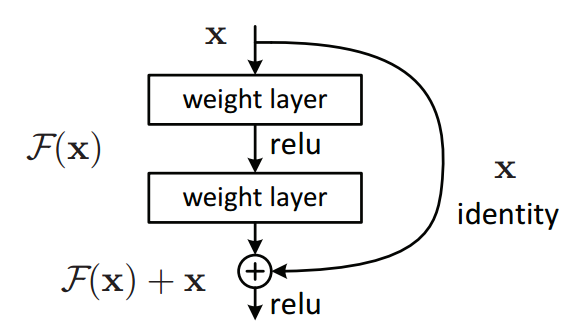
\includegraphics[width=1\linewidth]{images/residual_neuron.png}
	\caption{A residual neuron used in ResNet architecture showing the identity function skipping a connection.}
	\label{fig:residual}
\end{figure}

\begin{figure}[ht]
	\centering
	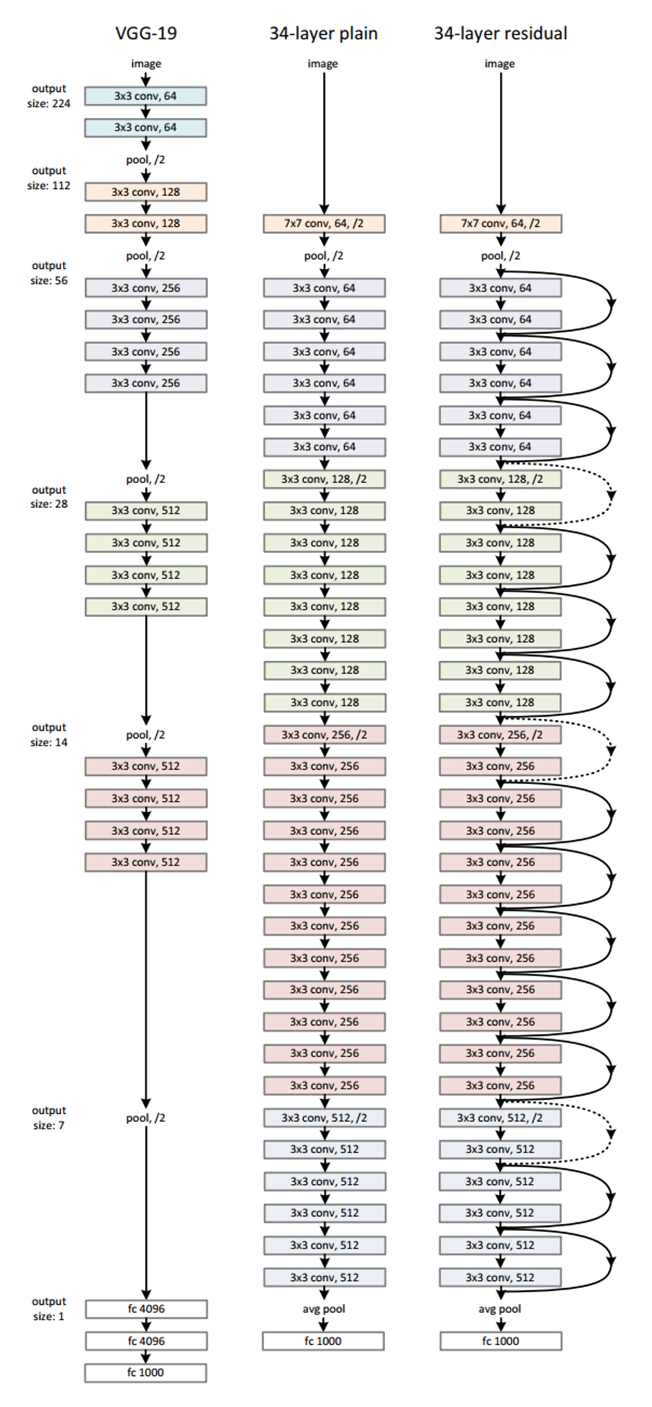
\includegraphics[width=0.8\linewidth]{images/resnet_full.png}
	\caption{A residual network in comparison to VGG-$19$ network and a $34$-layer non-residual network.}
	\label{fig:resnet_full}
\end{figure}


To explain this residual step formally, He {\it et al} \cite{He} use the following equations to describe the residual block over a few stacked layers:

\begin{equation}
    y = \mathcal{F}(x.\{W_i\}) + x
\end{equation}

where $x$ and $y$ are the input and outputs and the function $\mathcal{F}(x.\{W_i\})$ is the learned mapping. 

This equation holds for all layers where the dimensions of $x$ and $\mathcal{F}$ are the same. If they are different, for instance when reducing channels, the function is modified slightly to add a linearly projected matching parameter $W_s$:

\begin{equation}
    y = \mathcal{F}(x.\{W_i\}) + W_s x
\end{equation}

It can be seen from these equations that there is no difference between a residual network and a plain network in terms of depth, width, and number of parameters, and only a negligible difference in computation due to the element-wise addition.

The authors of this paper \cite{He} compared the residual networks (of differing depths up to 1000 layers) with 'plain' networks, VGG-$16$, GoogLeNet, PReLU-net, and BN-inception and found that ResNet's ability performed at up to $8\times$ deeper than VGG-$16$, but with less complexity. The results outperformed other networks when classifying ImageNet and CIFAR-$10$, as well as a $28\%$ improvement on COCO object detection. An ensemble of ResNets achieved $3.37\%$ error rate winning first prize in the ILSVRC 2015 classification task.


\subsection{Logistic Regression Classifier}

Linear->logistic regression explanation....


Mathematically, Resnet uses a 1000-way Softmax activation function to evaluate the output of the sum of all neurons:

\begin{equation}
\hat{Z} = SoftMax\Bigg \{ \sum_{n=0}^{N-1} \mathcal{F}(x.\{W_i\}) + W_s x \Bigg \}
\end{equation}

where $\hat{Z}$ is a 1000-length vector of probabilities associated with the input image. As the output layer is removed in our method, the penultimate layer vector ($\hat{X}$) is represented as the term inside the parenthesis:

\begin{equation}
\hat{X} = \sum_{i=0}^{N-1} \mathcal{F}(x.\{W_i\}) + W_s x
\end{equation}

with $N$ inputs, resulting in the feature vector $\hat{X}=[X_0, X_1, X_2,..., X_n]$. Training the Logistic Regression model, we maximise the probability:

\begin{equation}
P(\hat{X}) = \frac{1}{1+e^{-t_X}} 
= \frac{1}{1+e^{-(\beta_0+\beta_1 X_0 + \beta_2         X_1+...+\beta_m X_n)}}
\end{equation}

returning a vector of learned regression coefficients $\hat{\beta}=[\beta_0, \beta_1, \beta_2,...,\beta_m]$ which can be used as a model evaluate new data. 





%%%%%%%%%%%%%%%%%%%%%%%%%%%%%%%%%%



%%%%%%%%%%%%%%%%%%%%%%%%%%%%%%%%%%%%%%%%%%%%%%%%%%%%%%%%%%%%%%%%%%%%%%%%

\section{Generalisation}


In order to test the generalisability of this method, a comparison of different datasets was undertaken. The data was acquired from publicly available websites and trained using the Resnet-LR classification method. Objects in the datasets were chosen based on texture, colour and shape as determining factors in successful classification where intensity, scale and background were consistent. The first dataset chosen was a fruit classification task with 83 classes including Apples, Banana, Cherry, Clementine, Guava, Lemon, Orange, Peach, Strawberry and Tomato, and was created by Muresan and Oltean \cite{muresan} (https://www.kaggle.com/moltean/fruits). The fruit images are well scaled and background is removed to leave only the single fruit visible (Figure \ref{fig:fruits}).


\begin{figure}[ht]
	\centering
	\begin{subfigure}{0.45\linewidth}
		\centering
		\includegraphics[width=0.9\textwidth]{images/fruit1.jpg}
		\caption{}
		\label{fig:fr1}
	\end{subfigure}%
	\begin{subfigure}{0.45\linewidth}
		\centering
		\includegraphics[width=0.9\textwidth]{images/fruit2.jpg}
		\caption{}
		\label{fig:fr2}
	\end{subfigure}%
	
	\begin{subfigure}{0.45\linewidth}
		\centering
		\includegraphics[width=0.9\textwidth]{images/fruit3.jpg}
		\caption{}
		\label{fig:fr3}
	\end{subfigure}%
	\begin{subfigure}{0.45\linewidth}
		\centering
		\includegraphics[width=0.9\textwidth]{images/fruit4.jpg}
		\caption{}
		\label{fig:fr4}
	\end{subfigure}%
	
	\caption{(a)Red Banana, (b)Apple, (c)Pineapple, and (d)Pear fruits from the Fruits-360 dataset.}
	\label{fig:fruits}
\end{figure}



Muresan and Oltean \cite{muresan} developed the dataset and constructed and trained their own Convolutional Neural Network (CNN) in order to perform the classification task. Their best two results for testing are listed in Table \ref{tab:gen_results} showing the HSV method ($97.01\%$ testing accuracy), and a method using HSV, Greyscale, Hue and Saturation adjustments and augmenting ($97.04\%$ testing accuracy). Applying our Resnet-LR method, an accuracy of $97.50\%$ was achieved, improving on the scores the authors of the paper, showing the adaptable nature of this method.

The second dataset consists of flower species downloaded from the University of Oxford (http://www.robots.ox.ac.uk/\textasciitilde{} vgg/data/flowers/102/) and contains images of various wild flowers from across the UK. There are 102 classes (between 40 and 208 samples of each class) including fire lily, ball moss, monkshood, sweet pea, sunflower, desert-rose, and marigold (Figure \ref{fig:flowers}). The images have noisy backgrounds compared to the previous datasets as well as varying illumination, scale and occlusions. However, the algorithm still performed quite well achieving 93.39\% compared to the best score of 95.34\%.

\begin{figure}[ht]
	\centering
	\begin{subfigure}{0.45\linewidth}
		\centering
		\includegraphics[width=0.9\textwidth]{images/flower1.jpg}
		\caption{}
		\label{fig:fl1}
	\end{subfigure}%
	\begin{subfigure}{0.45\linewidth}
		\centering
		\includegraphics[width=0.9\textwidth]{images/flower2.jpg}
		\caption{}
		\label{fig:fl2}
	\end{subfigure}%
	
	\begin{subfigure}{0.45\linewidth}
		\centering
		\includegraphics[width=0.9\textwidth]{images/flower3.jpg}
		\caption{}
		\label{fig:fl3}
	\end{subfigure}%
	\begin{subfigure}{0.45\linewidth}
		\centering
		\includegraphics[width=0.9\textwidth]{images/flower4.jpg}
		\caption{}
		\label{fig:fl4}
	\end{subfigure}%
	
	\caption{Examples from the Oxford Flower dataset.}
	\label{fig:flowers}
\end{figure}




\begin{figure}[ht]
	\centering
	\begin{subfigure}{0.45\linewidth}
		\centering
		\includegraphics[width=0.9\textwidth]{images/obj1.png}
		\caption{}
		\label{fig:coil1}
	\end{subfigure}%
	\begin{subfigure}{0.45\linewidth}
		\centering
		\includegraphics[width=0.9\textwidth]{images/obj12.png}
		\caption{}
		\label{fig:coil2}
	\end{subfigure}%
	
	\begin{subfigure}{0.45\linewidth}
		\centering
		\includegraphics[width=0.9\textwidth]{images/obj66.png}
		\caption{}
		\label{fig:coil3}
	\end{subfigure}%
	\begin{subfigure}{0.45\linewidth}
		\centering
		\includegraphics[width=0.9\textwidth]{images/obj100.png}
		\caption{}
		\label{fig:coil4}
	\end{subfigure}%
	
	\caption{Examples from the COIL-100 dataset.}
	\label{fig:coil_images}
\end{figure}



Finally, the third dataset is the Columbia Object Image Library (COIL-100) consisting of 100 classes of everyday objects photographed at pre-determined angles on a turntable resulting in 72 images per class (total 7200). Some examples are shown in Figure \ref{fig:coil_images}, whilst Figure \ref{fig:coil_plot} shows the results of the experiment we performed that split the training and test sets into varying difficulty. Starting from a single, randomly selected (pose) training image per class (100 images), and the rest of the dataset is used as testing (7100 images). The number of samples per class was increased and the results visualise how quickly the accuracy converged to 100\%. This occurred at exactly the halfway point where 3600 images were used for both training and testing to give a perfect result. As shown in the graph, even with only one training image per class, at a random pose results in 78.5\% accuracy indicating Resnet's ability to extract features quickly and easily that can determine the differences between object classes with great accuracy. 



\begin{figure}
	\centering
	\includegraphics[width=0.9\linewidth]{images/COIL_graph.png}
	\caption{Plotting the accuracy of the COIL-100 dataset vs number of training images per class using our method.}
	\label{fig:coil_plot}
\end{figure}


These three problems do not have the fine-gained, defect detection characteristics of the strawberry problem, but show the general adaptability of this method to object classification. Furthermore, each of these classifiers is multi-class dependant opposed to the binary classifiers developed for the system. 




%\newpage
\section{Real-time Production Line Implementation}

Since agriculture began, it has relied on humans to perform quality assessment or separate produce into different grades, or to remove defects. These processes are diminished by many variations such as subjectivity of operators, human error, poor process, lack of training and under-staffing. These factors can result in huge variations in the quality of produce being shipped to customers, and as a result can incur extra costs by way of stock returns, reduced price point, and impacts on reputation.

Many agricultural farmers are beginning to adopt machine vision and automated control systems \cite{saldana} - \cite{costa} to help process their produce, giving them added confidence, greater control and efficiency, and reductions in rejected stock from customers. In the case of fruit and vegetables, supermarkets and boutique sellers of produce expect near perfect quality in terms of shape, size, texture, colour, as well as being free from visible (and invisible) defects such as disease and pest contamination. Smaller markets, outlets and retailers do not enforce such strict requirements, but do still maintain a good level of quality. This means that the best quality produce will often go to large customers who buy in bulk and will pay more for the best quality, whereas smaller markets will generally purchase cheaper grades with lower (but still acceptable) quality. However, market availability and weather conditions also contribute to the sales mix, where very good quality produce could potentially be impossible to supply or, conversely, has flooded the market.

In order to standardise the grading and detect defects in strawberries, this method has been implemented on a real-time production line. It extends work and construction by Eaton et al \cite{eaton1}, \cite{eaton2} who developed the in-line integration, conveyors, acquisition, lighting, and power systems as well as accumulating a data collection, and colour analysis methods.


The system is placed in-line with the strawberry packing line bottleneck where the multiple packing benches converge, or at the feed point for manually fed lines. This ensures that all strawberry punnets flow into the inspection system for assessment, are sealed in the automated sealing machine, and then palletised for transportation. The conveyors are controlled independently of the inspection system so as not to inhibit production rate. 


\subsection{System Configuration}

In order to keep production rates high, the pre-packed containers must be assessed as they arrive at the acquisition system, and ejected from the line if defected. During production, up to two strawberry punnets are packed per second (or $120/min$), largely determined by the number of packers employed and their proficiency levels, allowing only $500ms$ to process each punnet. The system developed by Eaton et al \cite{eaton1} has been designed to have a robust structure, due to its placement on the production floor, and is equipped with safety systems, signals, and controls interface for operator use. A cross section of the system and its major components are shown in Figure \ref{fig:full_system}. The system enclosure is made from $5mm$ stainless steel sheeting bolted to a $40mm$ aluminum frame. The enclosure houses all electronics and computing hardware required for sensing punnets, perform acquisitions, and controlling the system. 


\subsection{Image Acquisition}

Images are acquired by four FLIR Blackfly cameras with $1920\times 1200$ resolution and images transferred via USB3 to a PC. With two cameras above and two below the transparent punnet, the top and bottom of the fruits in the punnet can be thoroughly inspected, minimising the chance of defective berries hidden from the view of the cameras. The two pairs of cameras above and below comprise of both visible colour (RGB) and invisible Near Infrared (NIR).



\begin{figure}[ht]
	\centering
	\begin{subfigure}{.45\textwidth}
		\centering
		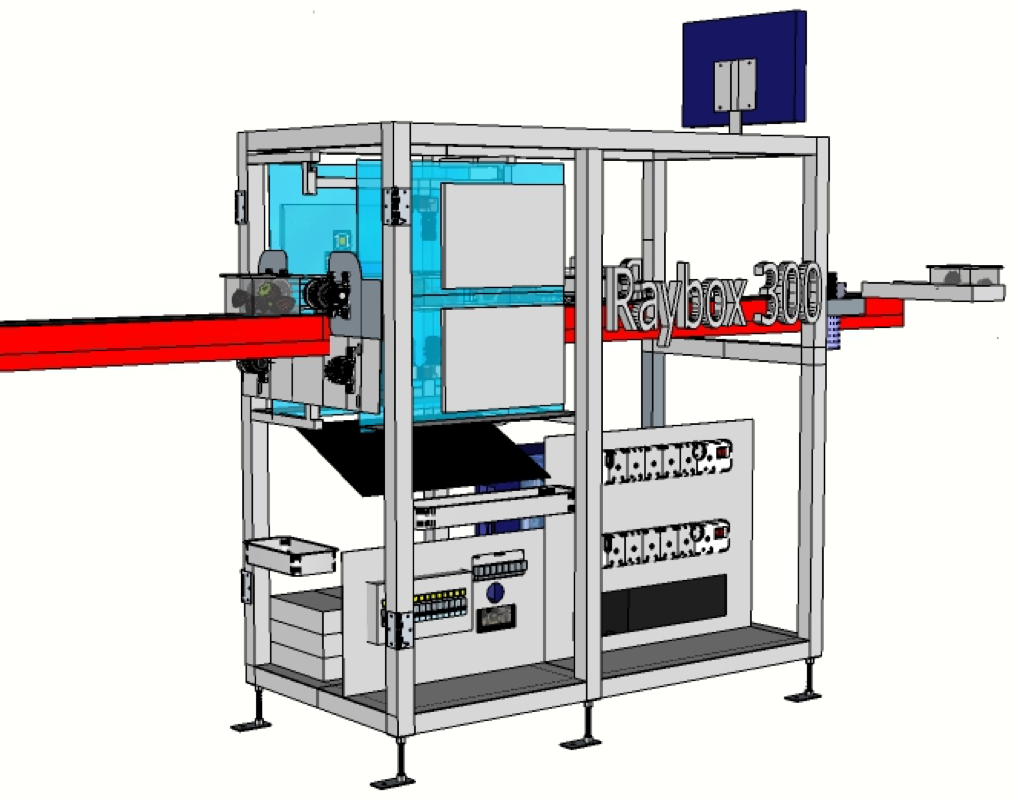
\includegraphics[width=1\linewidth]{images/SQA_v2.png}
		\caption{}
		\label{fig:enclosure_cross_sec}
	\end{subfigure}%
	
	\begin{subfigure}{.45\textwidth}
		\centering
		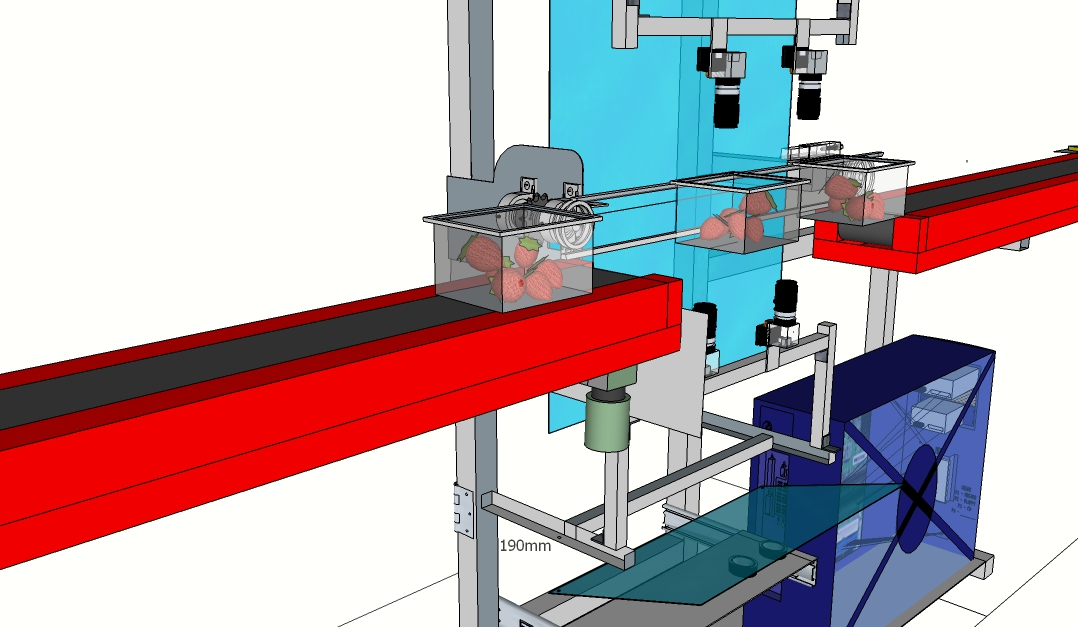
\includegraphics[width=1\linewidth]{images/QAS_cross_sec.jpg}
		\caption{}
		\label{fig:close_up_cross_sec}
	\end{subfigure}%
	
	\caption{Top: Components of the full system - conveyors, diffuser panels and polarisers, as well as electronic/computer storage. Bottom: Close up view of the v-belt conveyor subsystem and the camera set up. }
	\label{fig:full_system}
\end{figure}


The visible lighting is provided by $8 \times 100W$ chip-on-board (COB) LED devices (Fig. \ref{fig:LED_vis}) on both top and bottom of the punnet imaging conveyor. They each contain $100 \times 1W$ LED's and therefore generate heat quickly, they are commonly coupled with cooling devices in order to reduce thermal damage. The Colour Rendering Index (CRI) of these lighting devices are $>90\%$ meaning they have a wide spectral band as shown in Figure \ref{fig:LED_response}.

With the high speed of the punnet conveyor, images must be acquired in less than $4ms$ to avoid motion blur and at a rate of two punnets per second, hence the active acquisition time is less than $8ms$. This means the image acquisition does not require constant lighting but rather transient flashes. This strobing mechanism allows the top and bottom LEDs to be turn on and off alternatively in order to avoid backlighting and acquire clear fruit images of both the top and the bottom. This also means that there is no requirement for cooling given the $~1\%$ duty cycle, which has greatly reduced the complexity of the light subsystem and its power requirements.

Compared to other fruits such as apples and bananas, the surface structure of strawberries is unique, in the sense each seed is embedded in a funnel-shaped pit lower than the strawberry surface. Such structure creates ring-shaped glare (specular reflection) around every seed under direct light. In the worst case scenario, more than half of the surface inspected is covered by glare, effectively 'blinding' the computer vision algorithms where these reflections exist. In order to reduce glare, the diffuser panels and polarisers are employed (blue sheets in Figure \ref{fig:enclosure_cross_sec}).

\begin{figure}[ht]
	\centering
	\begin{subfigure}{.45\textwidth}
		\centering
		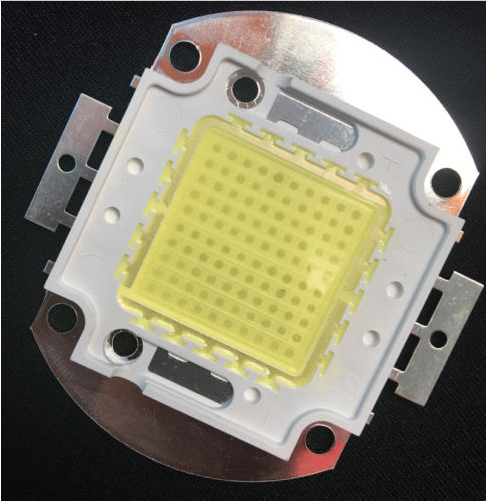
\includegraphics[width=0.7\linewidth]{images/LED_vis.png}
		\caption{}
		\label{fig:LED_vis}
	\end{subfigure}%
	
	\begin{subfigure}{.45\textwidth}
		\centering
		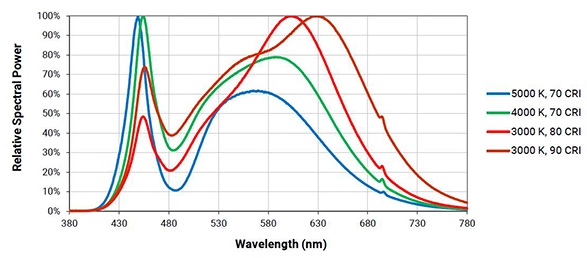
\includegraphics[width=1\linewidth]{images/LED_response.png}
		\caption{}
		\label{fig:LED_response}
	\end{subfigure}%
	
	\caption{Top: $100W$ LED chip on board device. Bottom: Response curves of the visible LEDs attained with different colour temperatures. }
	\label{fig:LED}
\end{figure}


\subsection{Data Collection}

A colour analysis method was implemented to demonstrate the system, and test the defect ejector. This method used HSV and CIELab colour spaces to extract the over ripe and under ripe areas by colour \cite{eaton2}, and was used for several months whilst collecting data. This data collection phase was required to generate data that was otherwise non-existant in order to train classifiers based on classical machine learning approach, e.g. regression analysis, as well as more advanced deep neural networks (DNN). During this phase, more than $100,000$ punnets were acquired and saved in a database, after which the labelling process commenced. The images were labelled in a binary manner as either pass or fail, with very little pre-processing and no segmentation given the fixed background and location of punnets in the camera view. Table \ref{tab:data} shows the data collected for training and testing purposes. Challenges in such colour analysis method include sensitivity to illumination changes, different cultivars of strawberries having different colour signatures, as well as confusions caused by colour similarities between under ripe berries and certain type of foreign objects, such as yellow calyx. In order to handle these challenges, a deep learning framework is adopted.




\subsection{Strawberry Classification}
\label{sec:strawberry_classification}



\begin{table*}\sffamily
	\caption{Example strawberry training images - Pass fruit (1), Under ripe fruit (2), Over ripe fruit (3), Foreign objects (4))}
	\label{tab:examples}
	\begin{tabular}{l*8{N}@{}}
		\toprule
		
		1 &
		\includegraphics[width=\linewidth]{images/pass_1.jpg} & \includegraphics[width=\linewidth]{images/pass_2.jpg} & \includegraphics[width=\linewidth]{images/pass_3.jpg} &         \includegraphics[width=\linewidth]{images/pass_4.jpg} & \includegraphics[width=\linewidth]{images/pass_5.jpg} &         \includegraphics[width=\linewidth]{images/pass_6.jpg} & \includegraphics[width=\linewidth]{images/pass_7.jpg} &         \includegraphics[width=\linewidth]{images/pass_8.jpg} \\
		
		2 &
		\includegraphics[width=\linewidth]{images/under_1.jpg} & \includegraphics[width=\linewidth]{images/under_2.jpg} & \includegraphics[width=\linewidth]{images/under_3.jpg} &         \includegraphics[width=\linewidth]{images/under_4.jpg} & \includegraphics[width=\linewidth]{images/under_5.jpg} &         \includegraphics[width=\linewidth]{images/under_6.jpg} & \includegraphics[width=\linewidth]{images/under_7.jpg} &         \includegraphics[width=\linewidth]{images/under_8.jpg} \\
		
		3 &
		\includegraphics[width=\linewidth]{images/over_1.jpg} & \includegraphics[width=\linewidth]{images/over_2.jpg} & \includegraphics[width=\linewidth]{images/over_3.jpg} &         \includegraphics[width=\linewidth]{images/over_4.jpg} & \includegraphics[width=\linewidth]{images/over_5.jpg} &         \includegraphics[width=\linewidth]{images/over_6.jpg} & \includegraphics[width=\linewidth]{images/over_7.jpg} &         \includegraphics[width=\linewidth]{images/over_8.jpg} \\
		
		4 &
		\includegraphics[width=\linewidth]{images/foreign_1.jpg} & \includegraphics[width=\linewidth]{images/foreign_2.jpg} & \includegraphics[width=\linewidth]{images/foreign_3.jpg} &         \includegraphics[width=\linewidth]{images/foreign_4.jpg} & \includegraphics[width=\linewidth]{images/foreign_5.jpg} &         \includegraphics[width=\linewidth]{images/foreign_6.jpg} & \includegraphics[width=\linewidth]{images/foreign_7.jpg} &         \includegraphics[width=\linewidth]{images/foreign_8.jpg} \\
		
		
		\bottomrule
	\end{tabular}
\end{table*} 



Captured images in Table \ref{tab:examples} shows the intensity, backgound and scale attributes are constant while the colour, edges and geometric attributes are variable yet finite (confined within the punnet), therefore the problem is a fine-grained classification task. However, the similarities between each strawberry image are much higher than that of other more general datasets (for example Oxford Flowers or Stanford Dogs where each image does not have a static background, scale or illumination). Therefore, such high level of similarity makes the classification task more challenging, calling for more robust feature descriptors that able to capture the distinctiveness in between different punnet categories (pass, overripe, underripe and those containing foreign objects).

It has been observed that, due to colour tone and reflection differences, examples of overripe strawberry punnets usually have lower overall pixel intensity than examples of underripe strawberry punnnets. However, such pixel intensity, which is mainly affected by the illumination condition, can also be indirectly affected by other factors, such as the way of packing. For example, how individual berries are positioned in the punnet (at random or uniformly arranged), average size of individual berries that determines the total surface area which in turn subsequently determines reflection and illumination. Therefore, we intentionally change the illumination conditions during the image acquisition process to ensure that our training examples include sufficient example images under different illumination conditions, hence making the deep learning instance robust against illumination variances.

The strawberry problem domain relates strongly to the colour and texture aspects of early-layer neural network feature extraction. As ResNet is a deep-learned network, trained on millions of object images making up $1000$ classes, we theorise (with further evidence provided by Pan {\it et al} \cite{pan}, Bianchini and Scarselli \cite{bianchini}) that it will detect more intricate differences in fine-grained object images due to its complexity, discriminating more easily between slight colour and texture variations. Also, this architecture provides a more efficient network propagation for real-time applications due to the residual elements.



\begin{table*}
	\centering
	\caption{Comparison of training results for commonly used classifiers against all three classes using identical feature vectors extracted from ResNet.}
	\label{tab:classifiers}
	\begin{tabularx}{0.85\textwidth}{ccccccc}
		\toprule
		& Foreign object &          & Under ripe    &          & Over ripe     &           \\  
		Classifier & Accuracy (\%)  & Log Loss & Accuracy (\%) & Log Loss & Accuracy (\%) & Log Loss  \\ 
		\midrule
		K-Neighbors Classifier          & 89.9297  & 1.2688 & 80.4989 & 1.4785 & 79.9550 & 1.4162 \\[6pt] 
		Logistic Regression	            & \textbf{96.9555}  & \textbf{0.0840} & \textbf{97.9592} & \textbf{0.0664} &  \textbf{99.3243} & \textbf{0.0445} \\[6pt]
		SVM (RBF)	                    & 51.5222  & 0.2976 & 47.1655 & 0.3754 & 47.5225 & 0.6921 \\[6pt]
		NuSVM	                        & 93.4426  & 0.1853 & 96.3719 & 0.1092 & 98.4234 & 0.0445 \\[6pt]
		Decision Tree Classifier	    & 89.4614  & 3.6399 & 80.9524 & 6.5788 & 83.3333 & 5.7565 \\[6pt]
		Random Forest Classifier	    & 90.6323  & 0.4432 & 83.4467 & 0.4808 & 87.8378 & 0.3963 \\[6pt]
		AdaBoost Classifier	            & 96.7213  & 0.5742 & 97.7324 & 0.5472 & 97.2973 & 0.5809 \\[6pt]
		MLP Classifier	                & 95.7845  & 0.2315 & 95.6916 & 0.2222 & 52.4775 & 0.6920 \\[6pt]
		Gradient Boosting Classifier	& 94.8478  & 0.1451 & 97.9592 & 0.0714 & 98.1982 & 0.0638 \\[6pt]
		Gaussian NB	                    & 53.8642  & 15.934 & 60.3175 & 13.7059 & 57.2072 & 14.7801 \\[6pt]
		Linear Discriminant Analysis	& 94.1452  & 0.2143 & 90.0227 & 0.4015 & 93.2432 & 0.3401 \\[6pt]
		Quadratic Discriminant Analysis	& 59.2506  & 14.0743 & 50.7937 & 16.9953 & 52.4775 & 16.4137 \\[6pt]
		\bottomrule 
	\end{tabularx}
\end{table*}





The method discussed in this paper is based on feature vector classification previously used in, for example, SVM, Random Forrest, and Regression techniques which are well-known classification methods. However, the feature vector that is classified in this case is generated by the ResNet neural network and its deep learned features. The network weights are not changed, or fine-tuned, as with previously mentioned methods, rather the penultimate layer vectors are used to train a classifier to recognise defects. 

The originally acquired images include a background of conveyor belts and other mechanical parts of the system, they also include top-bottom view of the sensor, its reflector and the entire punnet borders (in the top view) and the bottom of the punnet (in the bottom view). Since the location of the punnet in the camera field of view is fixed at each moment of capture and all punnets are of exactly the same size, the valid punnet region is cropped from the original acquired image with a fixed size of $500 \times 600$. 


Using a combination of horizontal and vertical flipping, images were compiled for training and listed in Table \ref{tab:data}.


\begin{table}[h]
	\centering
	\caption{Images collected and labelled for each class for testing and training.}
	\label{tab:data}
	\begin{tabular}{c c c c c} 
		\hline
		& Foreign & Under ripe & Over ripe & Pass \\ [0.5ex] 
		\hline
		Training & 1595 &  3542 & 4954 &  5412 \\
		Testing & 500 & 500 & 500 & 500 \\ [1ex] 
		\hline
	\end{tabular}
\end{table}



During the research and training phase, $12$ different classifiers were assessed for accuracy including K-Neighbours, AdaBoost, and SVM algorithms with results shown in Table \ref{tab:classifiers}. They were trained with respect to three defect classes namely, under ripe, over ripe, and foreign object, and indicate that simple Logistic Regression analysis is the best performing. 


Interestingly, the SVM with RBF kernel algorithm scored a very low $51.5\%$ while the NuSVM algorithm scored much higher at $93.4\%$ when comparing on the under ripe category. The difference between the these two methods are the $C$ and $Nu$ regularization parameters which apply penalties in the case of mis-classifications. The $C$ parameter used in SVC, ranges $\{\exists C\in\mathbb{Q^+}\}$ where $\mathbb{Q^+}$ is the set of positive rational numbers, meaning it can take any real value from zero to infinity. The $Nu$ parameter is limited to a range from zero to one only $\{\exists C\in\mathbb{Q} \mid 0 <\mathbb{Q} < 1\}$ and therefore, is bounded to search within a defined smaller range. 

The difference in these two scores indicates for this problem, the classifier will underfit using high-level parameters that can escalate infinitely. Therefore the Logistic Regression algorithm is used to classify the extracted strawberry features. 



%%%%%%%%%%%%%%%%%%%%%%%%%%%%%%%%%%



%%%%%%%%%%%%%%%%%%%%%%%%%%%%%%%%%%%%%%%%%%%%%%%%%%%%%%%%%%%%%%%%%%%%%%%%



\section{Application and results}




\begin{table}[ht]
	\centering
	\caption{Comparison of training and testing data with the Fruits-360 dataset using two best performing methods from Muresan and Oltean and our Logistic Regression model.}
	\label{tab:gen_results}
	\begin{tabular}{c c c c} 
		\hline
		Dataset & Team & Method & Testing  \\ [0.5ex] 
		\hline
		Fruits-360  & Muresan/Oltean    & CNN (HSV)                 & 97.01\% \\
		& Muresan/Oltean    & CNN (HSV+GS+HS+flips)     & 97.04\% \\
		& Ours              & Resnet + LogRes           & \textbf{97.50\%} \\ 
		\hline
		Oxford      & Simon/Rodner      & AlexNet const.            & 91.74\% \\
		Flowers     & VGG19             & Vanilla                   & 93.07\% \\
		& Ours              & Resnet + LogRes           & 93.39\% \\ 
		& Simon/Rodner      & VGG19 rand.               & 94.20\% \\
		& Simon/Rodner      & VGG19 const.              & \textbf{95.34\%} \\
		\hline
		COIL-100    & Matas/Obdrzalek   &                           & 94.7\% \\
		4 samples   & Maree et al       &                           & 95.28\% \\
		per class   & Chung et al       &                           & - \\
		& Ours              & Resnet + LogRes            & \textbf{96.01\%} \\
		
		\hline
		COIL-100    & Matas/Obdrzalek   &                           & - \\
		36 samples  & Maree et al       &                           & - \\
		per class   & Chung et al       &                           & 99.64\% \\
		&  Ours             & Resnet + LogRes            & \textbf{100.00\%}\\
		\hline
	\end{tabular}
\end{table}



The system is designed to acquire images at production time and pass them to the running application for assessment. The application is comprised of a GUI (to display statistics and detections to the operator), a controller to handle incoming images and signals, and outgoing signals, and an inference library which stores Resnet and classifier models.  


Given the independent classifier models and outcomes, the operator can increase the sensitivity of one of the defect classes while leaving the others unchanged, therefore allowing for the ability to adapt to changing weather and market conditions. 


For each image, Resnet needs only to produce a single feature vector that can then be predicted by each binary classifier to give a probability score. Although the structure of classifiers could be simplified by training one multi-class classifier, the independent fine-tuning during production would be lost. The operator is, therefore, able to make sensitivity adjustments in real-time by simply using a slider on the GUI. For example, the operator might adjust the confidence levels to $60\%, 90\%$, and $75\%$ for the foreign object, over ripe, and under ripe classes, respectively.

This then creates a subjective success measure, and due to this parameters variability, a Receiver Operating Characteristic (ROC) analysis  is performed with the results shown in Figure \ref{fig:ROCs}. The test images were acquired in real-time and then labelled retrospectively in order to obtain quantitative results.  

Both the Under Ripe and Foreign Object classifiers have performed well with the  Area Under ROC (AUROC) greater than $80\%$. However the Over Ripe classifier did not perform so well with an AUROC of $58\%$. This is most likely due to overfitting based on shadowed berries at the bottom of the punnet and could be overcome by pre-processing the data to contain only the top layer of fruit. This means that only fruit that is under full illumination will be classified as over ripe.

The other critical success factor was execution time, given that the production line requires two punnets per second to be acquired and assessed. Resnet has the ability to use its identity functions (discussed in Section \ref{sec:resnet}) which speeds up the propagation time of the network, and thus the inference is very fast. Without the use of a GPU, the entire process including the time taken for three classifiers averages $<300ms$, which is well within the given $500ms$ window.   




\begin{figure}[ht]
	\centering
	\begin{subfigure}{0.9\linewidth}
	    \centering
		\includegraphics[width=0.9\textwidth]{images/ROC_foriegn.png}
		\caption{}
		\label{fig:ROC_f}
	\end{subfigure}%
	
	\centering
	\begin{subfigure}{0.9\linewidth}
	    \centering
		\includegraphics[width=0.9\textwidth]{images/ROC_under.png}
		\caption{}
		\label{fig:ROC_u}
	\end{subfigure}%
	
	\begin{subfigure}{0.9\linewidth}
	    \centering
		\includegraphics[width=0.9\textwidth]{images/ROC_over.png}
		\caption{}
		\label{fig:ROC_o}
	\end{subfigure}%
	
	\caption{(a) ROC curve of the foreign object classifier. (b) ROC curve of the under ripe classifier. (c)ROC curve of the over ripe classifier.}
	\label{fig:ROCs}
\end{figure}







%%%%%%%%%%%%%%%%%%%%%%%%%%%%%%%%%%%


%%%%%%%%%%%%%%%%%%%%%%%%%%%%%%%%%%%%%%%%%%%%%%%%%%%%%%%%%%%%%%%%%%%%%%%%

\section{Conclusion}

As was theorised in Section \ref{sec:strawberry_classification}, the Resnet-LR method has excellent results analysing classification problems that rely on shape, texture and colour features to distinguish the classes. This method has been applied to the strawberry quality problem with good results in the Under Ripe and Foreign Object defect detection with AUROC of 80\% and 87\%, respectively. 

This method performed very well against three public datasets, namely, Fruits-360, Oxford Flowers 102 and COIL-100. The results show that this method is highly adaptable to problems that rely on colour, texture, and shape to distinguish classes.

\subsection{Future Work}

In order to improve the ROC curve, more labelled data is required to increase each classifiers performance, particularly the Over Ripe class. Further testing along with the addition of other defect classes, such as size and bruising, will be required once the data is gathered.    


%%%%%%%%%%%%%%%%%%%%%%%%%%%%%%%%%%%





% use section* for acknowledgement
\section*{Acknowledgment}





%%%%%%%%%%%%%%%%%%%%%%%%%%%%%%%%%%%



\bibliographystyle{ieeetr}
\begin{thebibliography}{1}
	
	%1
	\bibitem{saldana}
	Erick SALDAÑA, Raúl SICHE, Mariano LUJÁN, Roberto QUEVEDO, ``Review: computer vision applied to the inspection and quality control of fruits and vegetables'', {\em Brazil Journal of Food Technology}, DOI: 10.1590/S1981-67232013005000031, (2013).
	
	%
	\bibitem{bhargava}
	Anuja Bhargava, Atul Bansa, ``Fruits and vegetables quality evaluation using computer vision: A review'', {\em Journal of King Saud University - Computer and Information Sciences}, DOI: 10.1016 2018.06.002, (2018).
	
	%
	\bibitem{costa}
	Corrado Costa, Francesca Antonucci, Federico Pallottino, Jacopo Aguzzi, Da-Wen Sun, Paolo Menesatti, ``Shape Analysis of Agricultural Products: A Review of Recent Research Advances and Potential Application to Computer Vision'', {\em Food Bioprocess Technol}, No. 4, (2011) pp 673–692.
	
	%
	\bibitem{eaton1}
	G. Eaton, A. Busch, R. Bartels, Y. Gao, ``A Method To Create Stable Lighting And Remove Specular Reflections for Vision Systems'', {\em Digital Image Computing: Techniques and Applications (DICTA)}, DOI: 10.1109/DICTA.2017.8227392 (2017).
	
	%5
	\bibitem{eaton2}
	G. Eaton, A. Busch, R. Bartels, Y. Gao, ``Colour Analysis of Strawberries on a Real Time Production Line'', {\em Digital Image Computing: Techniques and Applications (DICTA)}, (2018).
	
	%
	\bibitem{liming}
	Xu Liming, Zhao Yanchao, ``Automated strawberry grading system based on image processing'', {\em Computers and Electronics in Agriculture}, 71S (2010) S32–S39.
	
	%
	\bibitem{bato}
	Pepito Menguito BATO et al, ``Study on Sorting System for Strawberry Using Machine Vision - Part 2'', {\em Journal of JSAM}, No. 62 (2), pp 101-110, 2000.
	
	%
	\bibitem{durand}
	A. Durand-Petiteville, S. Vougioukas, D.C. Slaughter, ``Real-time segmentation of strawberry flesh and calyx from images of singulated strawberries during postharvest processing'', {\em Computers and Electronics in Agriculture}, No. 142 (2017) pp 298–313.
	
	%
	\bibitem{hayashi}
	Shigehiko Hayashi et al, ``Evaluation of a strawberry-harvesting robot in a field test'', {\em Biosystems Engineering}, No. 105 (2010) pp 160–171.
	
	%10
	\bibitem{feng}
	Guo Feng, Cao Qixin and Nagata Masateru, ``Fruit Detachment and Classification Method for Strawberry Harvesting Robot'', {\em International Journal of Advanced Robotic Systems}, Vol. 5, No. 1 (2008) ISSN 1729-8806, pp 41-48.
	
	%
	\bibitem{yamamoto}
	Kyosuke Yamamoto, Seishi Ninomiya, Yoshitsugu Kimura, Atsushi Hashimoto, Yosuke Yoshioka, Takaharu Kameoka, ``Strawberry cultivar identification and quality evaluation on the basis of multiple fruit appearance features'', {\em Computers and Electronics in Agriculture}, No. 110 (2015) pp 233–240.
	
	%
	\bibitem{nagata}
	Masateru NAGATA, Jasper G. TALLADA, Taiichi KOBAYASH, ``Bruise Detection using NIR Hyperspectral Imaging for Strawberry (Fragaria x ananassa Duch.)'', {\em Environ. Control Biol}, No.  44 (2), pp 133-142, (2006).

	%
	\bibitem{benalia}
	Souraya Benalia, Sergio Cubero, José Manuel Prats-Montalbán, Bruno Bernardi, Giuseppe Zimbalatti, José Blasco, ``Computer vision for automatic quality inspection of dried figs (Ficus carica L.) in real-time'', {\em Computers and Electronics in Agriculture}, No. 120 (2016) pp 17–25.
	
	%
	\bibitem{arakeria}
	Megha.P.Arakeria, Lakshmana, ``Computer Vision Based Fruit Grading System for Quality Evaluation of Tomato in Agriculture industry'', {\em  Procedia Computer Science}, No. 79 (2016) pp 426–433 .

	%15
	\bibitem{yoon}
	Seung Chul Yoon, Bosoon Park, Kurt C. Lawrence, William R. Windham, Gerald W. Heitschmidt, ``Line-scan hyperspectral imaging system for real-time inspection of poultry carcasses with fecal material and ingesta'', {\em Computers and Electronics in Agriculture}, No. 79 (2011) pp 159–168.
	
	%
	\bibitem{keresztes}
	Janos C. Keresztes, Mohammad Goodarzi, Wouter Saeys, ``Real-time pixel based early apple bruise detection using short wave infrared hyperspectral imaging in combination with calibration and glare correction techniques'', {\em Food Control}, No. 66 (2016) pp 215-226.
	
	%
	\bibitem{coelho}
	Pablo A. Coelho, Sergio N. Torres, Wagner E. Ramírez, Pablo A. Gutierrez, Carlos A. Toro, Jose G. Soto, Daniel G. Sbarbaro, Jorge E. Pezoa, ``A machine vision system for automatic detection of parasites Edotea magellanica in shell-off cooked clam Mulinia edulis'', {\em Journal of Food Engineering}, No. 181 (2016) pp 84-91.
	
	%
	\bibitem{naik}
	Sapan Naik, Bankim Patel, ``Machine Vision based Fruit Classification and Grading - A Review'', {\em International Journal of Computer Applications}, Volume 170 – No.9, July 2017.
	
	%
	\bibitem{liu}
	Yuwei Liu, Hongbin Pu, Da-Wen Sun, ``Hyperspectral imaging technique for evaluating food quality and safety during various processes: A review of recent applications'', {\em Trends in Food Science \& Technology}, No. 69 (2017) pp 25-35.
	
	%20
	\bibitem{sun}
	Ke Sun, Ying Li,  Jing Peng,  Kang Tu,  Leiqing Pan, ``Surface Gloss Evaluation of Apples Based on Computer Vision and Support Vector Machine Method'', {\em Food Anal. Methods}, No. 10 (2017) pp 2800–2806.
	
	%
	\bibitem{nouri}
	Hosein Nouri-Ahmadabadi, Mahmoud Omid, Seyed Saeid Mohtasebi, Mahmoud Soltani Firouz, ``Design, development and evaluation of an online grading system for peeled pistachios equipped with machine vision technology and support vector machine'', {\em INFORMATION PROCESSING IN AGRICULTURE}, No. 4 (2017) pp 333–341.
	
	%
	\bibitem{cubero}
	S. Cubero, N. Aleixos, F. Albert, A. Torregrosa, C. Ortiz, O. Garcı´a-Navarrete, J. Blasco, ``Optimised computer vision system for automatic pre-grading of citrus fruit in the field using a mobile platform'', {\em Precision Agric}, No. 15 (2014) pp 80–94.
	
	%
	\bibitem{sofu}
	M.M. Sofu, O. Er, M.C. Kayacan, B. Cetisli, ``Design of an automatic apple sorting system using machine vision'', {\em Computers and Electronics in Agriculture}, No. 127 (2016) pp 395–405.
	
	%
	\bibitem{moallum}
	Payman Moallem, Alireza Serajoddin, Hossein Pourghassem, ``Computer vision-based apple grading for golden delicious apples based on surface features'', {\em INFORMATION PROCESSING IN AGRICULTURE}, No. 4 (2017) pp 33–40.
	
	%
	\bibitem{gill}
	Jasmeen Gill, Akshay Girdhar, Tejwant Singh, ``A Hybrid Intelligent System for Fruit Grading and Sorting'', {\em  International Journal on Computer Science and Engineering (IJCSE)}, Vol. 9 No.05 May 2017 pp 257-265.
	
	%
	\bibitem{zhang}
	Baohua Zhang, Wenqian Huang, Jiangbo Li, Chunjiang Zhao, Shuxiang Fan, Jitao Wu, Chengliang Liu, ``Principles, developments and applications of computer vision for external quality inspection of fruits and vegetables: A review'', {\em  Food Research International}, Vol. 62 (2014) pp 326–343.
	
	%
	\bibitem{shin}
	Hoo-Chang Shin, Holger R. Roth, Mingchen Gao, Le Lu, Ziyue Xu, Isabella Nogues, Jianhua Yao, Daniel Mollura, and Ronald M. Summers, ``Deep Convolutional Neural Networks for Computer-Aided Detection: CNN Architectures, Dataset Characteristics and Transfer Learning'', {\em IEEE TRANSACTIONS ON MEDICAL IMAGING}, VOL. 35, NO. 5, MAY 2016.
	
	%
	\bibitem{girshick}
	Ross Girshick, Jeff Donahue, Trevor Darrell, and Jitendra Malik, ``Region-Based Convolutional Networks for Accurate Object Detection and Segmentation'', {\em IEEE TRANSACTIONS ON PATTERN ANALYSIS AND MACHINE INTELLIGENCE}, VOL. 38, NO. 1, JANUARY 2016.
	
	%
	\bibitem{He}
	Kaiming He, Xiangyu Zhang, Shaoqing Ren, Jian Sun, ``Deep Residual Learning for Image Recognition'', {\em Computer Vision and Pattern Recognition}, arXiv:1512.03385 [cs.CV].
	
	%25
	\bibitem{pan}
	Junting Pan, Elisa Sayrol, Xavier Giro-i-Nieto, Kevin McGuinness, Noel E. O'Connor, ``Shallow and Deep Convolutional Networks for Saliency Prediction'', {\em Computer Vision and Pattern Recognition (CVPR)},  2016, pp 598-606.
	
	%
	\bibitem{bianchini}
	Monica Bianchini, Franco Scarselli, ``On the Complexity of Neural Network Classifiers: A Comparison Between Shallow and Deep Architectures'', {\em IEEE TRANSACTIONS ON NEURAL NETWORKS AND LEARNING SYSTEMS}, VOL. 25, NO. 8, AUGUST 2014.
	
	%
	\bibitem{muresan}
	Horea Muresan, Mihai Oltean, ``Fruit recognition from images using deeplearning'', {\em Acta Univ. Sapientiae, Informatica}, VOL. 10,1 (2018) 26-42.
	
	%
	
	
	
	
	%
	
	
\end{thebibliography}



%%%%%%%%%%%%%%%%%%%%%%%%%%%%%%%%%%%%%%%%%%%%%%%%%%%%%%%%%%%%


% that's all folks
\end{document}